\frame{
    \frametitle{Metabolite identification} 
    
    % we do not measure the structure. 
    % we have to infer the structure from the spectra, unlike in sequencing. 
    
\begin{small}
\begin{itemize}
    \item Small molecules ($<$ 1000 Da) involved in biological processes
    \item Identification of metabolites present in a biological sample
%     \item Widely used analysis workflow: \alert<2>{Liquid chromatography (LC)} combined with \alert<3>{tandem mass spectrometry (MS/MS)}
    \item Widely used analysis workflow: Liquid chromatography (LC) combined with tandem mass spectrometry (MS/MS)
\end{itemize}
\end{small}
\vspace{0.5cm}
% \includegraphics<2>[width=\textwidth]{images/lc_concept.pdf}
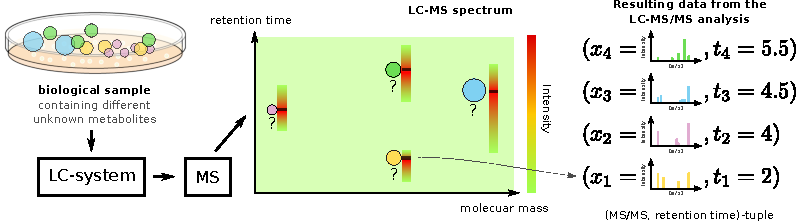
\includegraphics[width=\textwidth]{images/lcms_spectrum_complex_no_retention_order.pdf}
}

%% System LC vs Molecuar property MSMS

\frame{
    \frametitle{State-of-the-art MS/MS based metabolite identification} 

\begin{figure}[c]
    \centering
    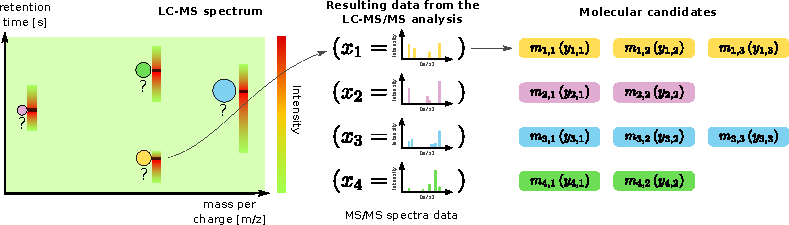
\includegraphics[width=1\textwidth]{images/lcms_spectrum_complex_small_only_iokr_with_candidates.pdf}
\end{figure}
\vspace{-0.15cm}
\begin{small}
\begin{block}{Identification workflow}
\vspace{-0.15cm}
\begin{enumerate}
    \item For each MS/MS spectra $x_i$ define a set of \emph{molecular candidate structures} $\{m_{i,1},m_{i,2},\ldots\}$.\hfill\ex{using the molecular mass}
    \item Assign a ``MS/MS matching score'' $y_{i,j}$ to each candidate.\\\hfill\ex{Input-Ouput-Kernel-Regression\cite{Brouard2016}}
    \item Higest scoring candidate $m_{i,j}$ is the identification for spectra $x_i$.
\end{enumerate}
\end{block}
\end{small}
}
